\documentclass[12pt]{article}

\usepackage{sbc-template}
\usepackage{graphicx,url}
\usepackage{multirow}
\usepackage[table,xcdraw]{xcolor}
\usepackage{lscape}
\usepackage{longtable}
\usepackage{pgfplots}
\pgfplotsset{width=10cm,compat=1.9}
\usepgfplotslibrary{external}
\tikzexternalize
\usepackage[utf8]{inputenc}
\usepackage[brazil]{babel}
\usepackage[latin1]{inputenc}  

\usepackage{listings}
\usepackage{color}

%New colors defined below
\definecolor{codegreen}{rgb}{0,0.6,0}
\definecolor{codegray}{rgb}{0.5,0.5,0.5}
\definecolor{codepurple}{rgb}{0.58,0,0.82}
\definecolor{backcolour}{rgb}{0.95,0.95,0.92}

%Code listing style named "mystyle"
\lstdefinestyle{mystyle}{
  backgroundcolor=\color{backcolour},   commentstyle=\color{codegreen},
  keywordstyle=\color{blue},
  numberstyle=\tiny\color{codegray},
  stringstyle=\color{codepurple},
  basicstyle=\footnotesize,
  breakatwhitespace=false,         
  breaklines=true,                 
  captionpos=b,                    
  keepspaces=true,                 
  numbers=left,                    
  numbersep=5pt,                  
  showspaces=false,                
  showstringspaces=false,
  showtabs=false,                  
  tabsize=2
}
\lstset{style=mystyle}
\sloppy

\title{Comparison of Path Planning Algorithms\\ }
\author{Karelia A. Vilca\inst{1}}

\address{Instituto de Ciências Matemáticas e de Computação -- Universidade de São Paulo
  (USP) \\ -- São Carlos, SP -- Brazil\\
  \email{\ karelia@usp.br}
}

\begin{document} 

\maketitle

\begin{abstract}

\end{abstract}

\section{Introduction}
Road planning is a widely investigated problem, there are multiple investigations such as robotics \cite{shwail2013probabilistic}, route optimization, etc. Likewise, there are different solution algorithms proposed, including informed and non-informed searches, as well as proposals that mix methods such as \cite{felner2003kbfs}.

The objective of the present work is to compare the performance of 4 algorithms, depth-first search, breadth-first search, A* and hill climbing applied in the road planning problem between two points. The implementation allows indicating a number of nodes and choosing between constructing a complete graph or not and provides the routes taken and details of time, cost, etc.

In this work some of the typical problems such as "Shortest path problem" and "Travel Salesman Problem" are explained. Next, two blind search algorithms and two heuristic algorithms are explained. Then implementation details are explained. And finally the results obtained are shown and compared.



\section{Path planning problems}
The routing problem is defined in terms of specified positions and transitions over links between them \cite{russell2004inteligencia}. 
To represent this type of problem, graphs or trees are used as data structures and the objective is achieved through search algorithms.
They can vary in the restriction of going through all the points or finding the direct route as the well-known road problem from Arad to Bucharest \cite{russell2004inteligencia}, likewise some methods find any possible way and others try to optimize finding the least expensive solution. Some of the problems are listed below.
\subsection{Shortest path problem}
Let $G =  (V, E)$ be a graph with  vertex  set $V$ of size $n$ and arc set $E$ of size $m$. Let $s$ be a distinguished  vertex  of $G$ and let c be a function  assigning a non negative  real valued cost to each arc of $G$. We denote the cost by $c(v,w)$. The single-source shortest path problem is that  of computing, for each vertex  $v$ reachable from  $S$, the cost of a minimum-cost  path  from  $s$ to  $v$ \cite{ahuja1990faster}. 

There are variations of this problem explained in \cite{dreyfus1969appraisal}; for example the shortest path problem between a specified pair of nodes or between all pair of nodes of a network. In 1959 Dijkstra \cite{dijkstra1959note} described The most efficient procedure  for for this problem. 

\subsection{Travel Salesman Problem}
\cite{little1963algorithm} describe this problem as s salesman, starting in one city, wishes to visit each of n-1 other cities and return to the start. In what order should he visit the cities to minimize the total distance traveled? Distance (time or cost) or costs between all city pairs are presumed known.

It is closely related to the hamiltonian-cycle problem and that's why it's considered NP-complete \cite{cormen2009introduction}. Reference \cite{bellmore1968traveling} discusses methods of solution including Dynamic Programming.

\section{Algorithms}
There are different algorithms for traversing or searching tree or graph data structures. For the search task, they can be grouped into blind search algorithms and algorithms of heuristic search.

\subsection{Blind Search Algorithms (Uninformed)}
According to \cite{russell2004inteligencia}, these strategies do not have additional information on states, as well as those provided by the definition of the problem. All search strategies are distinguished by the order in which we are expanded. An example shows DFS and BFS.

\subsubsection{Depth-first search (DFS)}
It was invented by Charles Pierre Trémaux (1859-1882) \cite{tremaux2010ecole} as a maze solving algorithm.
This algorithm implies, to search “deeper” in the graph whenever possible \cite{cormen2009introduction} and
considers the following choice rule: when selecting an
edge to traverse, always choose an edge emanating from the vertex most recently reached which still has unexplored edges \cite{tarjan1972depth}.
It is neither complete nor optimal, but it has linear spatial complexity \cite{russell2004inteligencia}.

In implementation terms it uses one LIFO stack, it means that the most recently generated node is chosen for expansion \cite{russell2004inteligencia}.

\lstinputlisting[language=C++, caption=DFS algorithm]{codes/DFS.hpp}
%\clearpage
\subsubsection{Breadth-first search (BFS)}
This method selects the shallow nodes for expansion; it is complete, great for unit cost steps, but it has exponential time complexity \cite{russell2004inteligencia}.
While the bradth search uses a FIFO, the depth search uses a LIFO. 
\lstinputlisting[language=C++, caption=BFS algorithm]{codes/BFS.hpp}

\subsection{Heuristic Search Algorithms (Informed)}
According to \cite{russell2004inteligencia},an informed search strategy uses knowledge of a specific problem in addition to the definition of the problem itself and can find solutions more efficiently than a search strategy without information. In the case of path problem, they know if a non-objective state is “more promising” than another.

\subsubsection{A*}
\lstinputlisting[language=C++, caption=A* algorithm]{codes/Aasterisk.hpp}

\subsubsection{Hill Climbing}
\lstinputlisting[language=C++, caption=Hill Climbing algorithm]{codes/HillClimbing.hpp}

\subsection{Comparison}
Following \cite{Maharshi2018ComparativeAO}, \cite{HLweb} and \cite{stuart2003artificial}, the performance of the algorithms can be compared based on the following parameters:
\begin{itemize}
    \item Time complexity: Time taken to find a solution.
    \item Space complexity: Memory required to perform the search.
    \item Optimality: Solution provided by the algorithm will always be optimal or not.
    \item Completeness: Always find the solution if it exists?
\end{itemize}
\begin{longtable}[c]{|c|c|c|c|c|}
\hline
\textbf{Algorithm}        & \textbf{DFS} & \textbf{BFS} & \textbf{A*} & \textbf{Hill Climbing} \\ \hline
\endhead
%
\textbf{Time Complexity}  & $O(b^{m})$   & $O(b^{d})$   & $O(b^{m})$  & $O(\infty)$            \\ \hline
\textbf{Space Complexity} & $O(bm)$      & $O(b^{d})$   & $O(b^{m})$  & $O(b^{m})$             \\ \hline
\textbf{Optimality}       & No           & Yes          & Yes         & No                     \\ \hline
\textbf{Completeness}     & No           & Yes          & Yes         & No                     \\ \hline
\caption{}
\label{tab:my-table}\\
\end{longtable}


\section{Implementation details}
\begin{lstlisting}[language=C++, caption=Build graph and tree]
void Build_graph()
{	
	//Empty matrix
	vector<float> vect;	
	for(int i=0; i<dots.size();i++)
		vect.push_back(0);	
	for(int i=0; i<dots.size();i++)
		grafo.push_back(vect);
	float d;
	//Adjacence matrix
	for(int i=0; i<dots.size();i++)
	{	vector<int> adj;
		for(int j=0; j<dots.size();j++)
		{   
			d=distance(dots[i].first,dots[j].first,dots[i].second,dots[j].second);
			if(d<limit)
			{
				grafo[i][j]=d;
				edges.push_back(make_pair(make_pair(dots[i].first,dots[i].second),make_pair(dots[j].first,dots[j].second)));///Grafico
				adj.push_back(j);
			}
		}
		graph.push_back(adj);
	}
}

void Build_tree()
{
	for(int i=0; i<dots.size();i++)
	{	
		vector<int> sons;
		for(int j=i; j<dots.size();j++)
		{
			if(grafo[i][j]<limit)
				sons.push_back(j);
		}
		tree.push_back(sons);
	}	
}
\end{lstlisting}
\begin{lstlisting}[language=C++, caption=Build graph and tree]
    cout<<"Number of dots"<<endl;
    cin>>N_DOTS;
    cout<<endl<<"Complete graph? (y/n)"<<endl;
    char yn;
    cin>>yn;
    if(yn=='n')limit=N_DOTS*0.8;
    cout<<endl<<"Press key to algorithm path"<<endl;
    cout<<"d ---> DFS "<<endl; 
    cout<<"b ---> BFS "<<endl;
    cout<<"a ---> A* "<<endl;
    cout<<"h ---> Hill Climbing "<<endl;
    
    srand(time(NULL));
    ///Random dots
    for(int i=0; i<N_DOTS; ++i)
    {
        float auxx=rand()%N_DOTS-rand()%N_DOTS;
        float auxy=rand()%N_DOTS-rand()%N_DOTS;
		dots.push_back(make_pair(auxx,auxy));
    }
    coord_ini=0;
    coord_fin=rand()%N_DOTS;
    start = dots[coord_ini];
    meta = dots[coord_fin];
    
    Build_graph();
    Build_tree();
  	Algorithms();
\end{lstlisting}
\subsection{Cost}
The cost of a path is the sum of the costs of its edges.\cite{ahuja1990faster}
\subsection{Visualization}

\begin{figure}[ht]
\centering
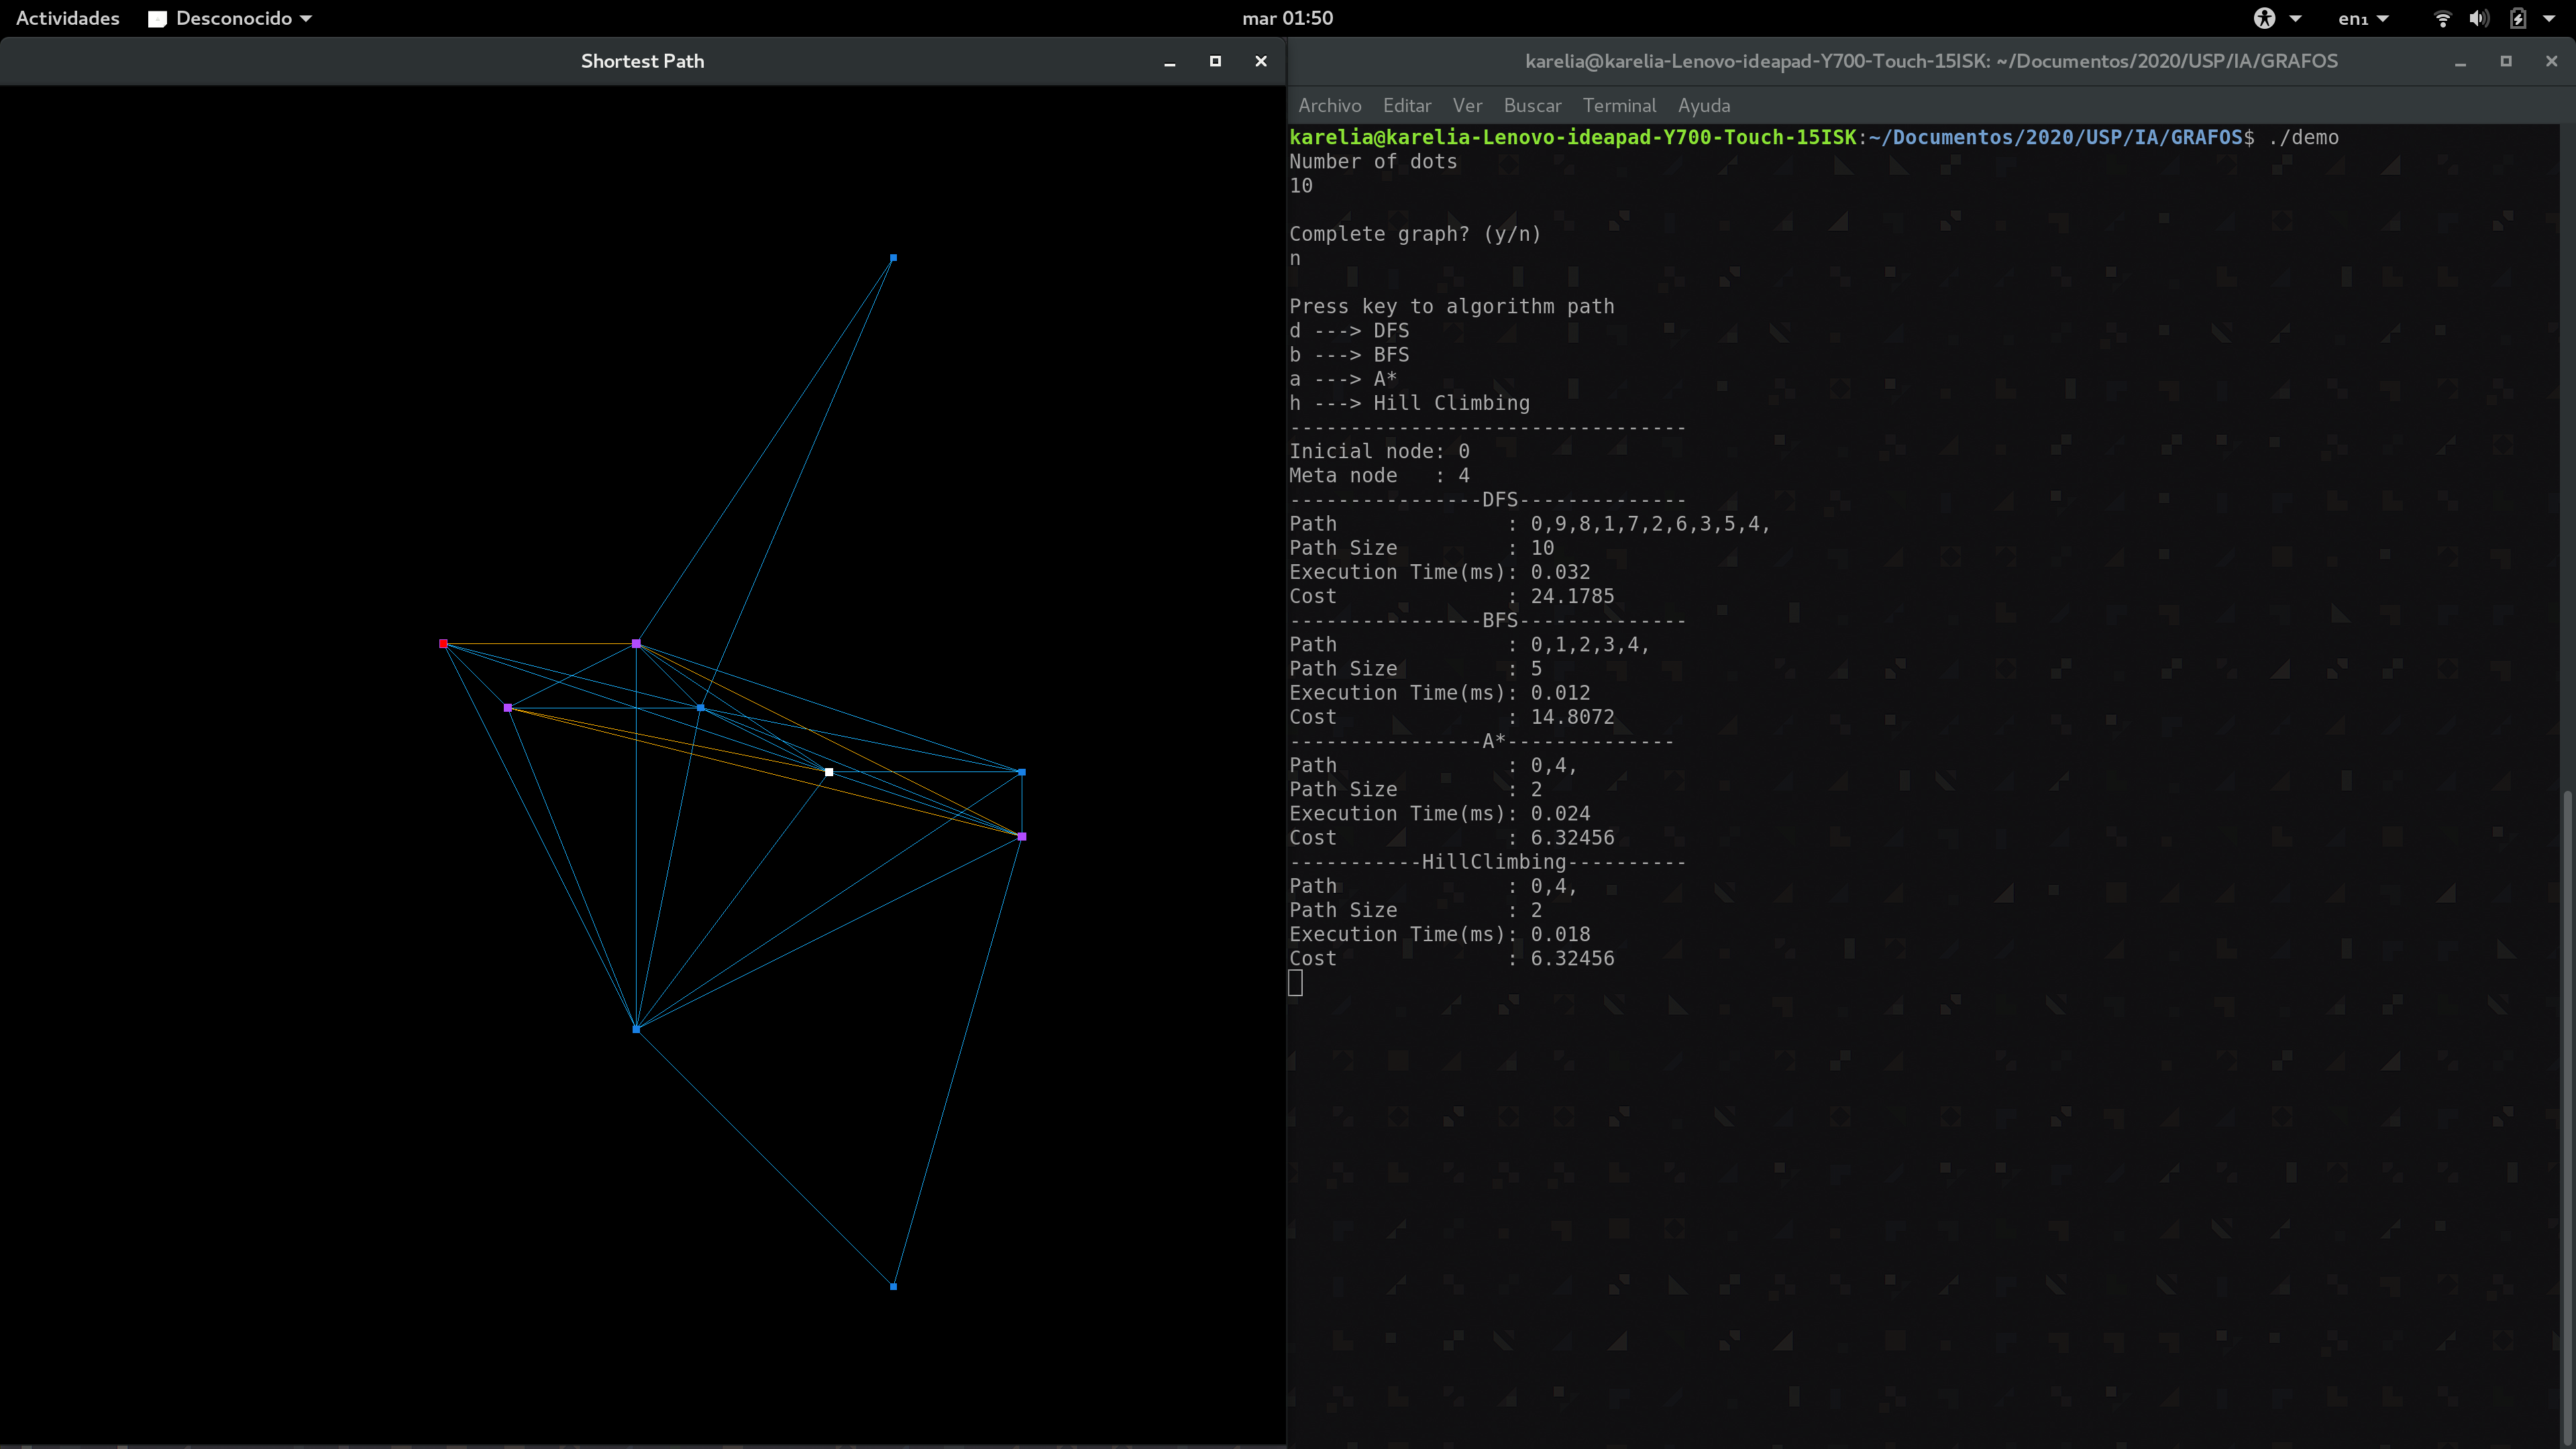
\includegraphics[width=1.0\textwidth]{Template_SBC/template-latex/screen1.png}
\caption{A typical figure}
\label{fig:exampleFig1}
\end{figure}

\begin{figure}[ht]
\centering
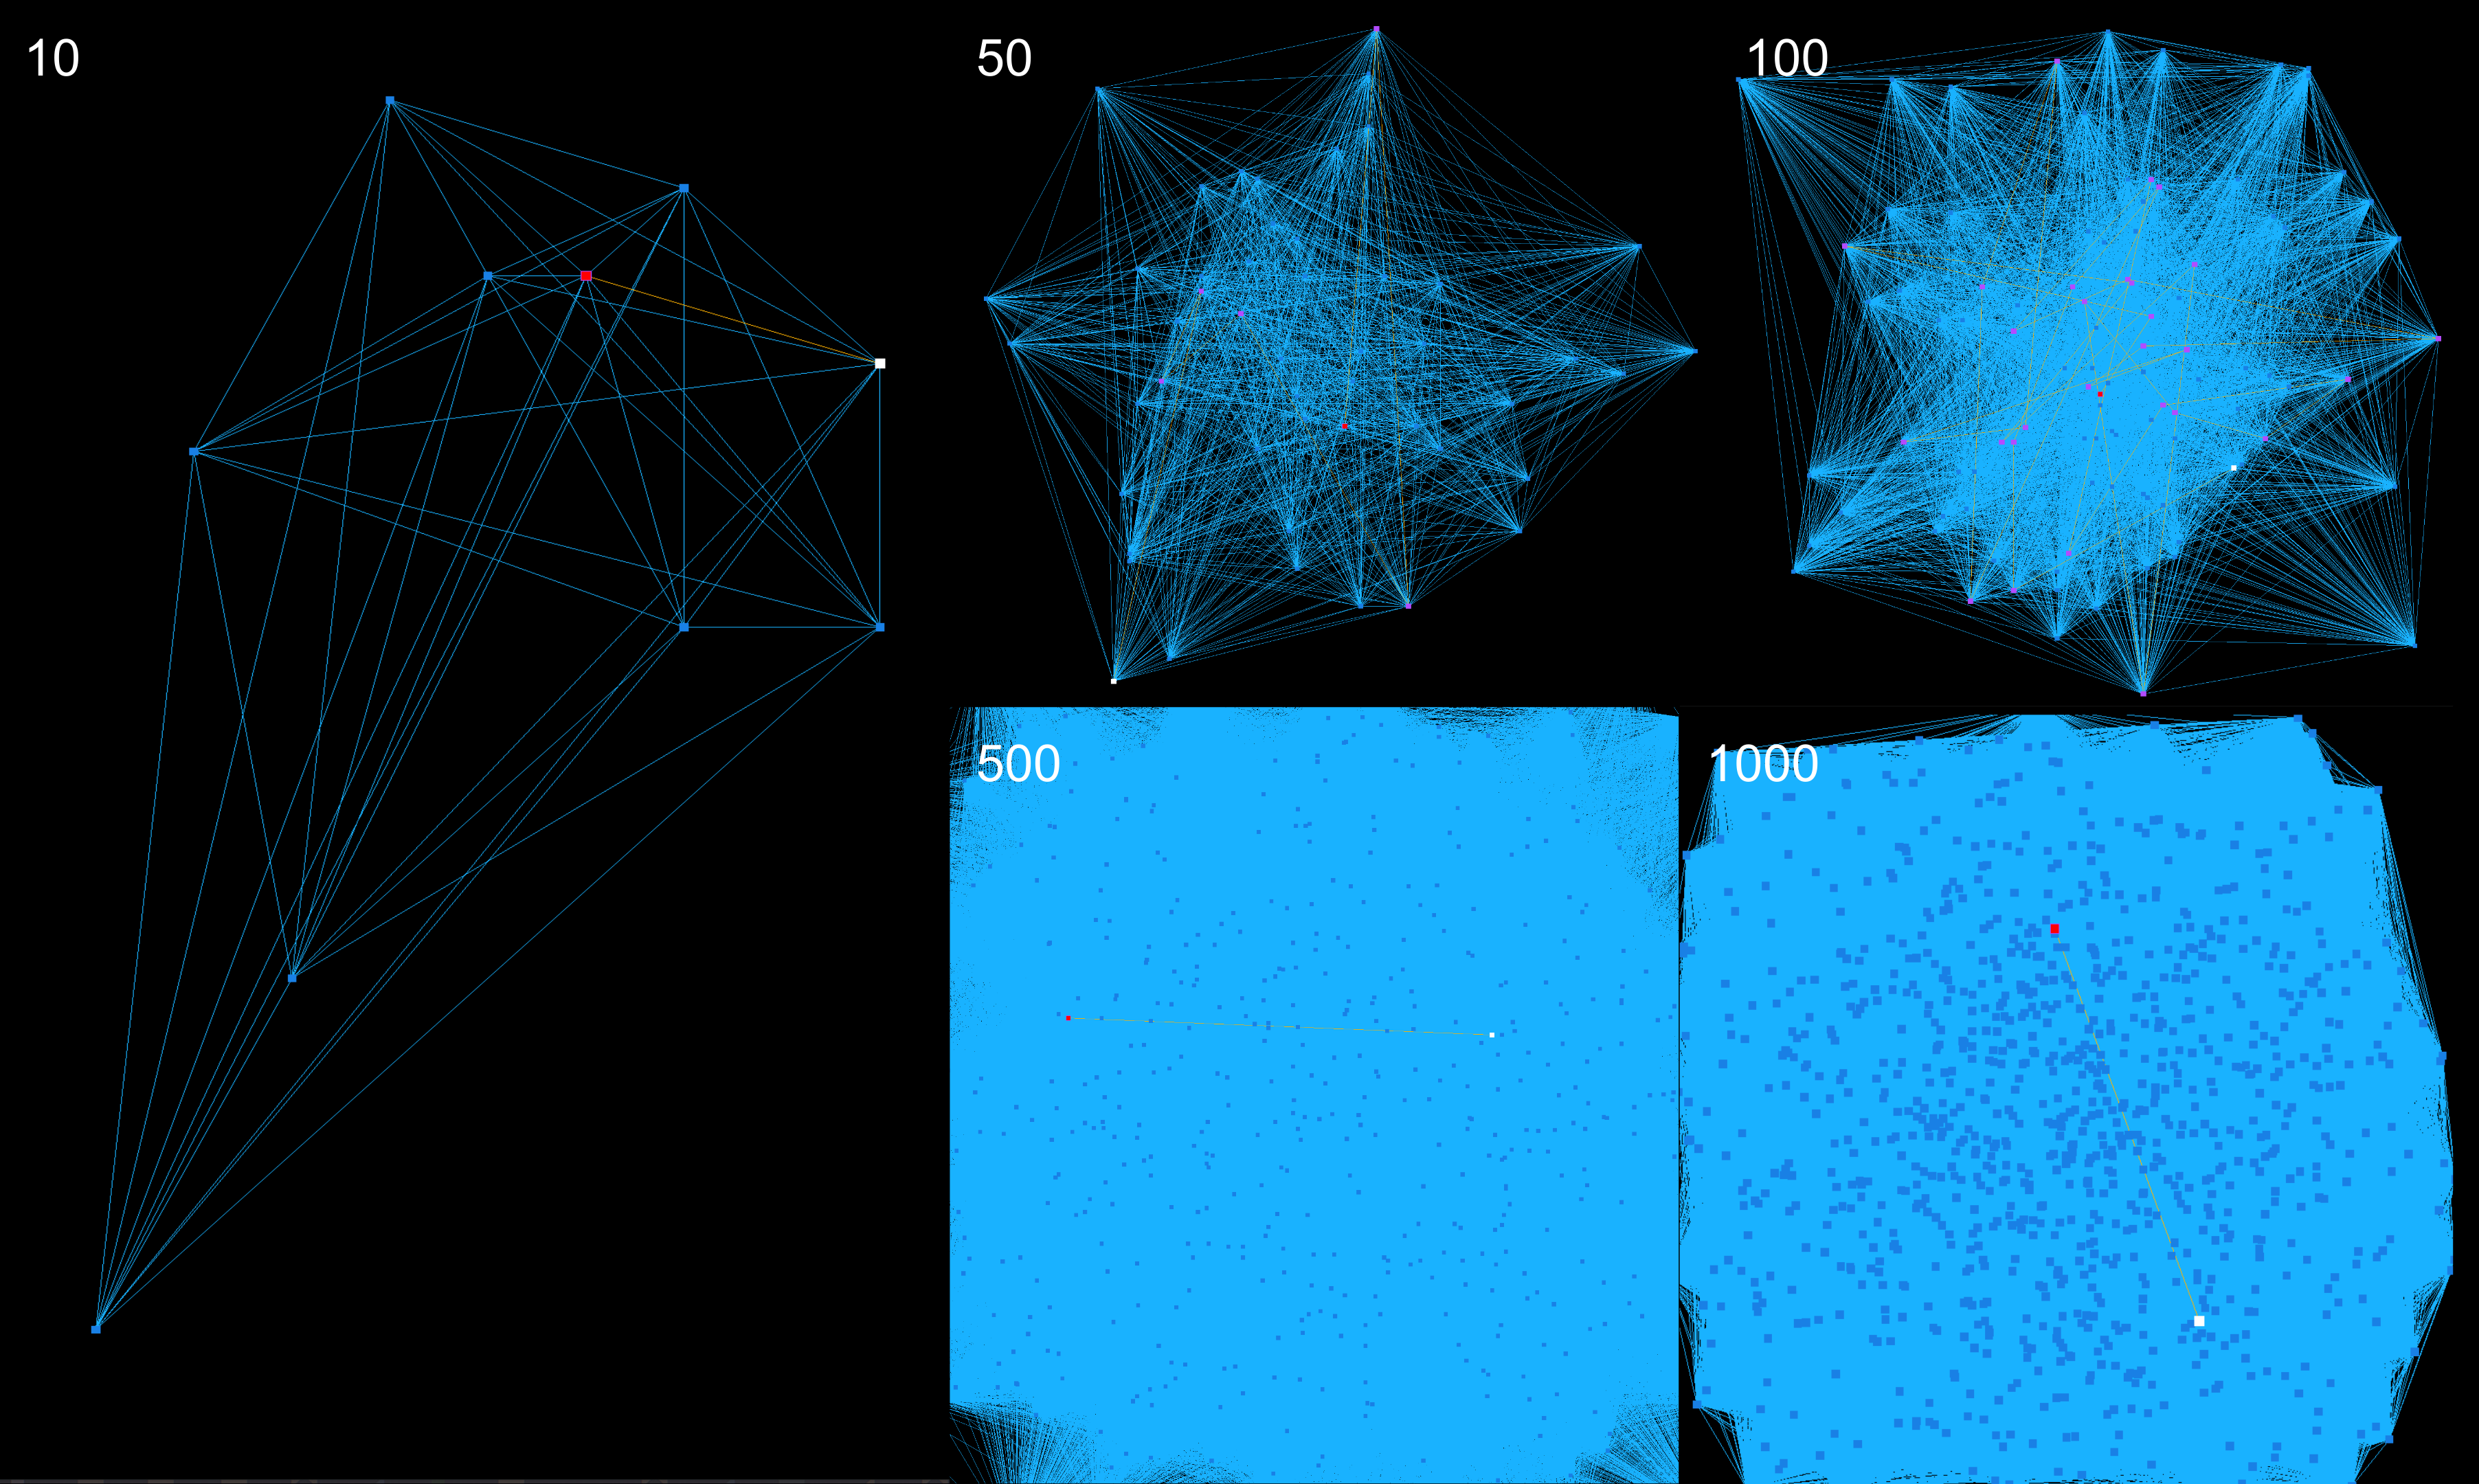
\includegraphics[width=1.0\textwidth]{Template_SBC/template-latex/grafoc.png}
\caption{This figure is an example of a figure caption taking more than one
  line and justified considering margins mentioned in Section~\ref{sec:figs}.}
\label{fig:exampleFig2}
\end{figure}

\begin{figure}[ht]
\centering
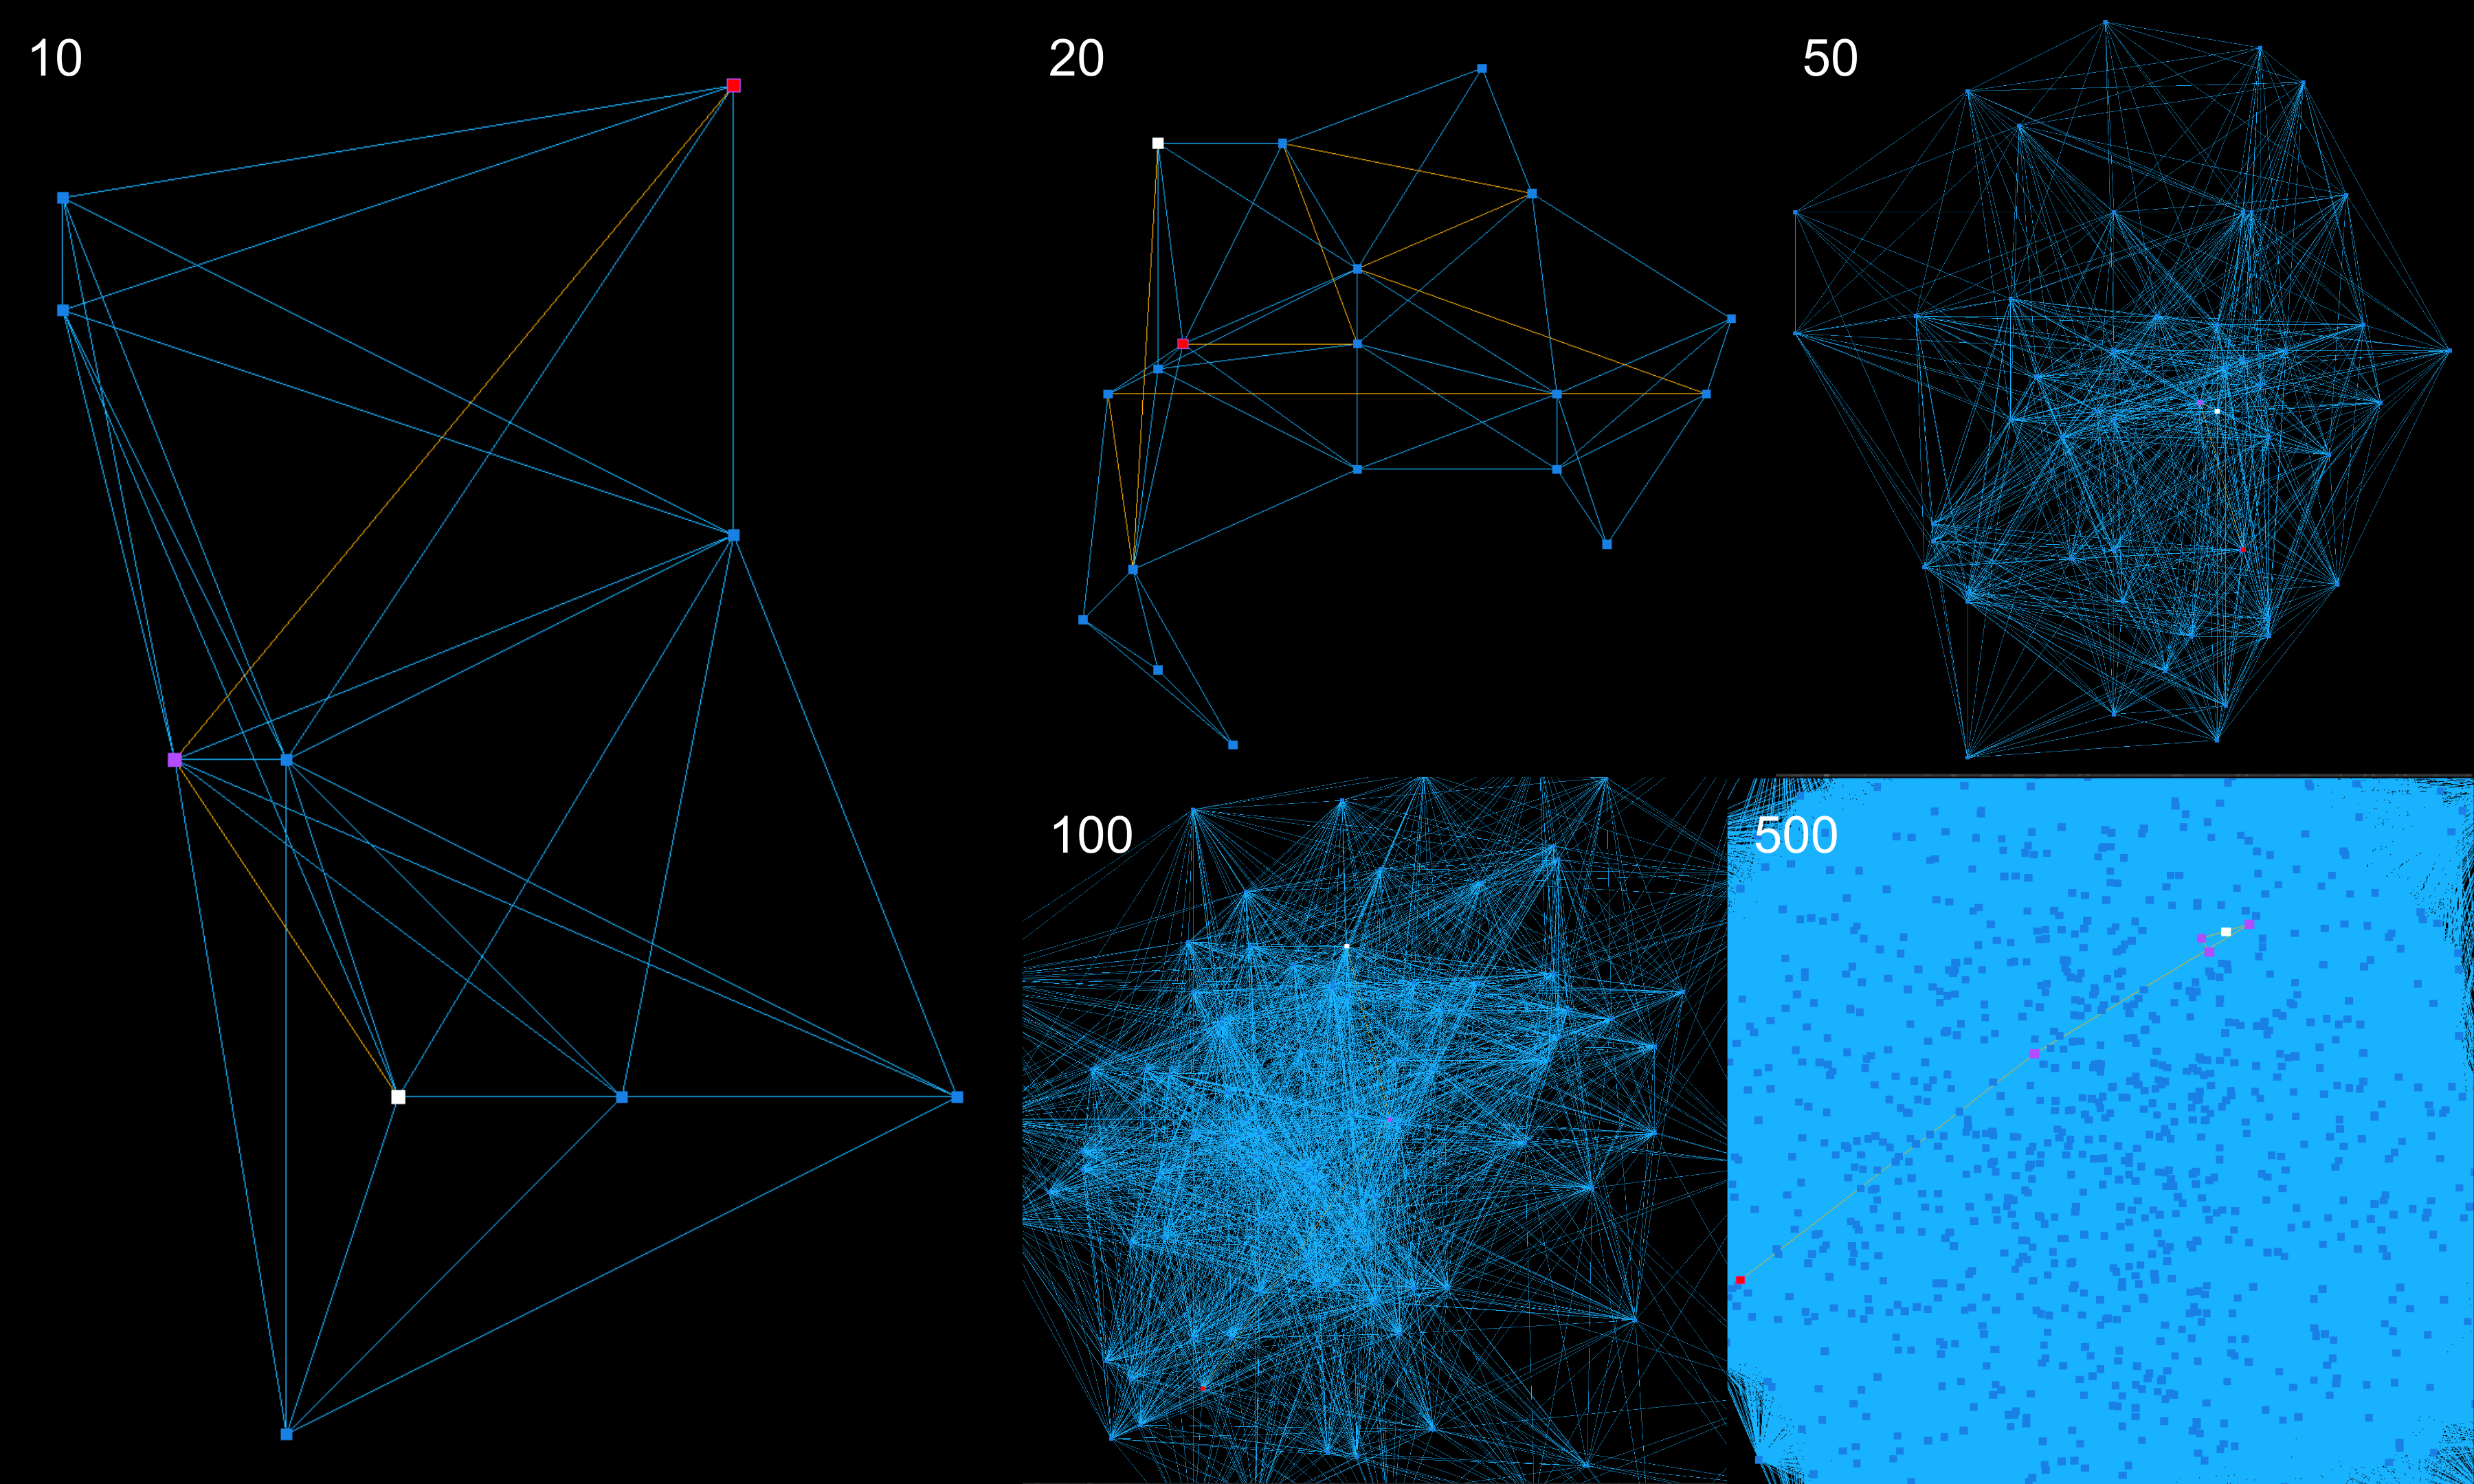
\includegraphics[width=1.0\textwidth]{Template_SBC/template-latex/grafonc.png}
\caption{This figure is an example of a figure caption taking more than one
  line and justified considering margins mentioned in Section~\ref{sec:figs}.}
\label{fig:exampleFig2}
\end{figure}


\section{Results}

\begin{landscape}
\begin{longtable}[c]{|c|c|l|l|l|l|l|l|l|l|l|l|l|l|}
\hline
\multicolumn{2}{|c|}{} &
  \multicolumn{6}{c|}{\textbf{Blind}} &
  \multicolumn{6}{c|}{\textbf{Heuristic}} \\ \cline{3-14} 
\multicolumn{2}{|c|}{\multirow{-2}{*}{\textbf{Search}}} &
  \multicolumn{3}{c|}{\textbf{DFS}} &
  \multicolumn{3}{c|}{\textbf{BFS}} &
  \multicolumn{3}{c|}{\textbf{A*}} &
  \multicolumn{3}{c|}{\textbf{Hill Climbing}} \\ \hline
\endhead
%
\multicolumn{2}{|c|}{\textbf{Features}} &
  \multicolumn{1}{c|}{} &
  \multicolumn{1}{c|}{} &
  \multicolumn{1}{c|}{} &
  \multicolumn{1}{c|}{} &
  \multicolumn{1}{c|}{} &
  \multicolumn{1}{c|}{} &
  \multicolumn{1}{c|}{} &
  \multicolumn{1}{c|}{} &
  \multicolumn{1}{c|}{} &
  \multicolumn{1}{c|}{} &
  \multicolumn{1}{c|}{} &
  \multicolumn{1}{c|}{} \\ \cline{1-2}
\textbf{\#N} &
  \textbf{Comp.} &
  \multicolumn{1}{c|}{\multirow{-2}{*}{\textbf{\begin{tabular}[c]{@{}c@{}}Path\\ size\end{tabular}}}} &
  \multicolumn{1}{c|}{\multirow{-2}{*}{\textbf{\begin{tabular}[c]{@{}c@{}}E.Time\\ (ms)\end{tabular}}}} &
  \multicolumn{1}{c|}{\multirow{-2}{*}{\textbf{Cost}}} &
  \multicolumn{1}{c|}{\multirow{-2}{*}{\textbf{\begin{tabular}[c]{@{}c@{}}Path\\ size\end{tabular}}}} &
  \multicolumn{1}{c|}{\multirow{-2}{*}{\textbf{\begin{tabular}[c]{@{}c@{}}E.Time\\ (ms)\end{tabular}}}} &
  \multicolumn{1}{c|}{\multirow{-2}{*}{\textbf{Cost}}} &
  \multicolumn{1}{c|}{\multirow{-2}{*}{\textbf{\begin{tabular}[c]{@{}c@{}}Path\\ size\end{tabular}}}} &
  \multicolumn{1}{c|}{\multirow{-2}{*}{\textbf{\begin{tabular}[c]{@{}c@{}}E.Time\\ (ms)\end{tabular}}}} &
  \multicolumn{1}{c|}{\multirow{-2}{*}{\textbf{Cost}}} &
  \multicolumn{1}{c|}{\multirow{-2}{*}{\textbf{\begin{tabular}[c]{@{}c@{}}Path\\ size\end{tabular}}}} &
  \multicolumn{1}{c|}{\multirow{-2}{*}{\textbf{\begin{tabular}[c]{@{}c@{}}E.Time\\ (ms)\end{tabular}}}} &
  \multicolumn{1}{c|}{\multirow{-2}{*}{\textbf{Cost}}} \\ \hline
 &
  \textbf{Y} &
  3 &
  0.022 &
  15.1333 &
  9 &
  0.02 &
  67.2523 &
  \cellcolor[HTML]{C0C0C0}2 &
  0.023 &
  \cellcolor[HTML]{C0C0C0}2.23607 &
  \cellcolor[HTML]{C0C0C0}{\color[HTML]{00009B} 2} &
  \cellcolor[HTML]{C0C0C0}{\color[HTML]{00009B} 0.19} &
  \cellcolor[HTML]{C0C0C0}{\color[HTML]{00009B} 2.23607} \\ \cline{2-14} 
\multirow{-2}{*}{\textbf{10}} &
  \textbf{N} &
  10 &
  0.032 &
  24.1785 &
  5 &
  \cellcolor[HTML]{C0C0C0}0.012 &
  14.8072 &
  \cellcolor[HTML]{C0C0C0}2 &
  0.024 &
  \cellcolor[HTML]{C0C0C0}6.32456 &
  \cellcolor[HTML]{C0C0C0}{\color[HTML]{00009B} 2} &
  \cellcolor[HTML]{FFFFFF}{\color[HTML]{00009B} 0.018} &
  \cellcolor[HTML]{C0C0C0}{\color[HTML]{00009B} 6.32456} \\ \hline
 &
  \textbf{Y} &
  7 &
  \cellcolor[HTML]{C0C0C0}0.055 &
  254.153 &
  47 &
  0.061 &
  1645.44 &
  \cellcolor[HTML]{C0C0C0}2 &
  0.086 &
  \cellcolor[HTML]{C0C0C0}44.6878 &
  \cellcolor[HTML]{C0C0C0}{\color[HTML]{00009B} 2} &
  {\color[HTML]{00009B} 0.08} &
  \cellcolor[HTML]{C0C0C0}{\color[HTML]{00009B} 44.6878} \\ \cline{2-14} 
\multirow{-2}{*}{\textbf{50}} &
  \textbf{N} &
  13 &
  0.067 &
  166.22 &
  44 &
  \cellcolor[HTML]{C0C0C0}0.045 &
  715.09 &
  \cellcolor[HTML]{C0C0C0}3 &
  0.07 &
  \cellcolor[HTML]{C0C0C0}19.9561 &
  \cellcolor[HTML]{C0C0C0}{\color[HTML]{00009B} 3} &
  {\color[HTML]{00009B} 0.063} &
  \cellcolor[HTML]{C0C0C0}{\color[HTML]{00009B} 19.9561} \\ \hline
 &
  \textbf{Y} &
  60 &
  0.151 &
  4375.48 &
  30 &
  \cellcolor[HTML]{C0C0C0}0.01 &
  1759.3 &
  \cellcolor[HTML]{C0C0C0}2 &
  0.038 &
  \cellcolor[HTML]{C0C0C0}39.4462 &
  \cellcolor[HTML]{C0C0C0}{\color[HTML]{00009B} 2} &
  {\color[HTML]{00009B} 0.033} &
  \cellcolor[HTML]{C0C0C0}{\color[HTML]{00009B} 39.4462} \\ \cline{2-14} 
\multirow{-2}{*}{\textbf{100}} &
  \textbf{N} &
  46 &
  0.104 &
  1439.16 &
  23 &
  \cellcolor[HTML]{C0C0C0}0.008 &
  650.663 &
  {\color[HTML]{036400} 4} &
  {\color[HTML]{036400} 0.039} &
  \cellcolor[HTML]{C0C0C0}{\color[HTML]{036400} 101.829} &
  \cellcolor[HTML]{C0C0C0}3 &
  0.034 &
  109.776 \\ \hline
 &
  \textbf{Y} &
  42 &
  0.454 &
  14382.9 &
  21 &
  \cellcolor[HTML]{C0C0C0}0.007 &
  8103.29 &
  \cellcolor[HTML]{C0C0C0}2 &
  0.592 &
  \cellcolor[HTML]{C0C0C0}432.334 &
  \cellcolor[HTML]{C0C0C0}{\color[HTML]{00009B} 2} &
  {\color[HTML]{00009B} 0.192} &
  \cellcolor[HTML]{C0C0C0}{\color[HTML]{00009B} 432.334} \\ \cline{2-14} 
\multirow{-2}{*}{\textbf{500}} &
  \textbf{N} &
  155 &
  1.681 &
  22679.9 &
  423 &
  \cellcolor[HTML]{C0C0C0}0.095 &
  61618.9 &
  {\color[HTML]{036400} 4} &
  {\color[HTML]{036400} 0.643} &
  \cellcolor[HTML]{C0C0C0}{\color[HTML]{036400} 295.431} &
  \cellcolor[HTML]{C0C0C0}{\color[HTML]{9A0000} 3} &
  {\color[HTML]{9A0000} 0.239} &
  {\color[HTML]{9A0000} 305.566} \\ \hline
 &
  \textbf{Y} &
  479 &
  8.333 &
  369845 &
  761 &
  \cellcolor[HTML]{C0C0C0}0.14 &
  561553 &
  \cellcolor[HTML]{C0C0C0}2 &
  1.694 &
  \cellcolor[HTML]{C0C0C0}1009.37 &
  \cellcolor[HTML]{C0C0C0}{\color[HTML]{00009B} 2} &
  {\color[HTML]{00009B} 0.693} &
  \cellcolor[HTML]{C0C0C0}{\color[HTML]{00009B} 1009.37} \\ \cline{2-14} 
\multirow{-2}{*}{\textbf{1000}} &
  \textbf{N} &
  375 &
  6.943 &
  106020 &
  813 &
  \cellcolor[HTML]{C0C0C0}0.153 &
  224880 &
  6 &
  1.98 &
  \cellcolor[HTML]{C0C0C0}1264.81 &
  \cellcolor[HTML]{C0C0C0}{\color[HTML]{036400} 5} &
  {\color[HTML]{036400} 0.783} &
  {\color[HTML]{036400} 1476.18} \\ \hline
 &
  \textbf{Y} &
  1840 &
  153.077 &
  6.80316e+06 &
  920 &
  \cellcolor[HTML]{C0C0C0}0.161 &
  3.258e+06 &
  \cellcolor[HTML]{C0C0C0}{\color[HTML]{00009B} 2} &
  {\color[HTML]{00009B} 51.328} &
  \cellcolor[HTML]{C0C0C0}{\color[HTML]{00009B} 2743.08} &
  \cellcolor[HTML]{C0C0C0}2 &
  55.802 &
  \cellcolor[HTML]{C0C0C0}2743.08 \\ \cline{2-14} 
\multirow{-2}{*}{\textbf{5000}} &
  \textbf{N} &
  3242 &
  258.704 &
  4.88624e+06 &
  1621 &
  \cellcolor[HTML]{C0C0C0}0.3 &
  2.49728e+06 &
  \cellcolor[HTML]{C0C0C0}{\color[HTML]{00009B} 3} &
  {\color[HTML]{00009B} 52.477} &
  \cellcolor[HTML]{C0C0C0}{\color[HTML]{00009B} 4391} &
  \cellcolor[HTML]{C0C0C0}3 &
  54.227 &
  4408.22 \\ \hline
 &
  \textbf{Y} &
  4537 &
  738.471 &
  3.29035e+07 &
  7732 &
  \cellcolor[HTML]{C0C0C0}1.367 &
  5.66735e+07 &
  \cellcolor[HTML]{C0C0C0}2 &
  194.085 &
  \cellcolor[HTML]{C0C0C0}9182.16 &
  \cellcolor[HTML]{C0C0C0}{\color[HTML]{00009B} 2} &
  {\color[HTML]{00009B} 193.342} &
  \cellcolor[HTML]{C0C0C0}{\color[HTML]{00009B} 9182.16} \\ \cline{2-14} 
\multirow{-2}{*}{\textbf{10 000}} &
  \textbf{N} &
  1503 &
  259.197 &
  4.30721e+06 &
  {\color[HTML]{036400} 9249} &
  \cellcolor[HTML]{C0C0C0}{\color[HTML]{036400} 1.519} &
  {\color[HTML]{036400} 2.68546e+07} &
  {\color[HTML]{9A0000} 6} &
  {\color[HTML]{9A0000} 208.628} &
  \cellcolor[HTML]{C0C0C0}{\color[HTML]{9A0000} 7755.03} &
  \cellcolor[HTML]{C0C0C0}{\color[HTML]{9A0000} 4} &
  {\color[HTML]{9A0000} 220.049} &
  {\color[HTML]{9A0000} 9006.27} \\ \hline
\multicolumn{2}{|l|}{\textbf{Average}} &
  \textbf{879.428} &
  \textbf{101.949} &
  \textbf{3529950.866} &
  \textbf{1549.857} &
  \cellcolor[HTML]{9B9B9B}{\color[HTML]{333333} \textbf{0.278}} &
  \textbf{6438884.838} &
  \textbf{3} &
  \textbf{36.550} &
  \cellcolor[HTML]{9B9B9B}{\color[HTML]{333333} \textbf{1949.121}} &
  \cellcolor[HTML]{9B9B9B}{\color[HTML]{333333} \textbf{2.642}} &
  \textbf{37.553} &
  \textbf{2056.114} \\ \hline
\caption{Table of results }
\label{tab:my-table}\\
\end{longtable}
\end{landscape}


\begin{tikzpicture}
\begin{axis}[
    ybar,
    enlargelimits=0.15,
    legend style={at={(0.5,-0.15)},
      anchor=north,legend columns=-1},
    ylabel={Average},
    symbolic x coords={DFS,BFS,A*,HC},
    xtick=data,
    nodes near coords,
    nodes near coords align={vertical},
    ]
\addplot coordinates {(DFS,879) (BFS,1549) (A*,3) (HC,2)};
\addplot coordinates {(DFS,101) (BFS,0.2) (A*,36) (HC,37)};
\addplot coordinates {(DFS,352) (BFS,643) (A*,0.1) (HC,0.2)};
\legend{Path size,E. Time(ms),Cost/1000}
\end{axis}
\end{tikzpicture}

\section{Conclusions}

\clearpage
\bibliographystyle{sbc}
\bibliography{sbc-template}

\end{document}
